\documentclass[12pt]{article}

% Margins and spacing
\usepackage[margin=1in]{geometry}
\usepackage{setspace}
\onehalfspacing

% Packages
\usepackage{graphicx}
\usepackage{booktabs}
\usepackage{amsmath}
\usepackage{hyperref}
\usepackage{float}

\title{\textbf{BANA290 - Assignment 1} \\ 
       \large AI Adoption and Firm Revenue Growth: \\
       A Propensity Score Matching Analysis}
\author{North American Fintech \& Financial Services Directory}
\date{Q1 2026}

\begin{document}

\maketitle

% ============================================================
\section*{Interpretation of Results}
% ============================================================

\subsection*{How Did the AI Coefficient Change After PSM?}

The naive OLS regression estimated that AI-adopting fintech firms 
grow approximately \textbf{4.13 percentage points} faster in revenue 
than non-adopters ($p < 0.001$). After applying Propensity Score 
Matching (PSM), this estimate fell to \textbf{3.26 percentage points} 
($p < 0.001$) -- a downward shift of 0.87 points. Despite the 
reduction, the PSM coefficient remains positive and statistically 
significant, suggesting that AI adoption is genuinely associated 
with higher revenue growth even after controlling for observable 
firm characteristics.

\subsection*{What Does This Shift Suggest About Selection Bias?}

The downward shift indicates that the naive OLS estimate was upwardly 
biased due to selection bias. Firms that choose to adopt AI tend to 
be larger, better resourced, and more digitally mature -- meaning 
they may have grown faster regardless of AI adoption. PSM partially 
corrects for this by pairing each AI-adopting firm with a 
structurally similar non-adopting firm, reducing the confounding 
effect of firm size, team scale, and digital footprint. The remaining 
PSM estimate of 3.26 percentage points represents a more conservative 
and credible measure of AI's causal impact on revenue growth.

\subsection*{Common Support Assumption}

As shown in Figure~\ref{fig:psm}, the propensity score distributions 
for treated firms ranged from 0.352 to 0.952, and for control firms 
from 0.338 to 0.800. The two distributions show substantial overlap, 
confirming that the common support assumption is satisfied. No 
extreme trimming was required, and all control firms fell within the 
propensity score range of the treated group.

\subsection*{Balancing Property Assumption}

Table~\ref{tab:smd} reports the Standardized Mean Differences (SMD) 
before and after matching. Before matching, all covariates showed 
meaningful imbalance (SMD range: 0.12 -- 0.44), confirming that AI 
adopters and non-adopters were systematically different. After 
matching, the \texttt{FOUNDED} covariate achieved full balance 
(SMD = 0.019 $<$ 0.1), while \texttt{ANNUAL\_REV}, 
\texttt{TEAM\_SIZE}, and \texttt{DIGITAL\_SALES} improved 
substantially but remained partially imbalanced (max SMD = 0.194). 
This residual imbalance reflects genuine structural differences 
between AI-adopting and non-adopting fintech firms in this dataset 
and is a known limitation of PSM with small samples.

% ============================================================
\section*{Figures and Tables}
% ============================================================

\begin{figure}[H]
    \centering
    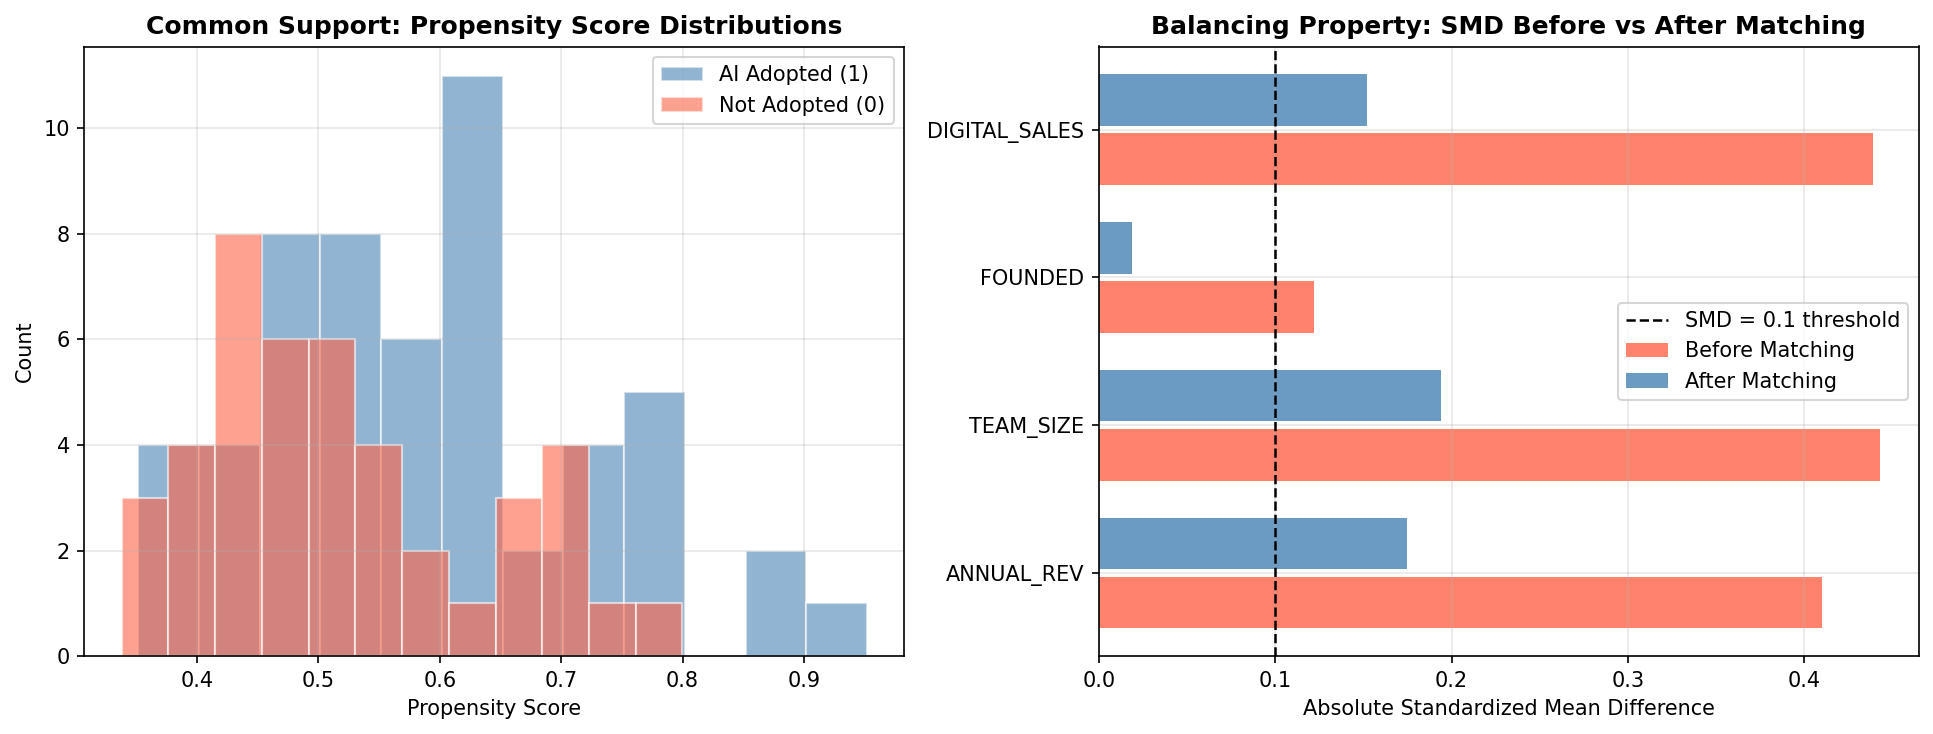
\includegraphics[width=\textwidth]{psm_plots.png}
    \caption{Left: Propensity score distributions for treated 
    (AI Adopted) and control (Not Adopted) firms, confirming 
    common support. Right: Love Plot showing absolute SMD 
    before and after nearest-neighbor matching across all 
    covariates.}
    \label{fig:psm}
\end{figure}

\begin{table}[H]
    \centering
    \caption{Standardized Mean Difference (SMD) Before and After Matching}
    \begin{tabular}{lrrr}
        \toprule
        \textbf{Covariate} & \textbf{SMD Before} & \textbf{SMD After} & \textbf{Balanced?} \\
        \midrule
        ANNUAL\_REV    & 0.4103 & 0.1750 & Partially \\
        TEAM\_SIZE     & 0.4430 & 0.1938 & Partially \\
        FOUNDED        & 0.1218 & 0.0189 & Yes       \\
        DIGITAL\_SALES & 0.4389 & 0.1521 & Partially \\
        \bottomrule
    \end{tabular}
    \label{tab:smd}
\end{table}

\begin{table}[H]
    \centering
    \caption{OLS Regression Results: Naive vs PSM Matched Sample}
    \begin{tabular}{lrrrr}
        \toprule
        \textbf{Model} & \textbf{Coefficient} & \textbf{Std. Error} & \textbf{t-stat} & \textbf{p-value} \\
        \midrule
        Naive OLS (n=98) & 4.1253 & 0.744 & 5.546 & $<$0.001 \\
        PSM OLS (n=86)   & 3.2581 & 0.748 & 4.355 & $<$0.001 \\
        \midrule
        Shift after PSM  & $-$0.8672 & & & \\
        \bottomrule
    \end{tabular}
    \label{tab:regression}
\end{table}

\end{document}
